\documentclass[a4paper]{report}
\usepackage{graphicx}
\usepackage{lscape}

\pagestyle{plain}

\usepackage{ exscale, latexsym, amsthm, amssymb, amsmath,hyperref,color, ifthen}
\usepackage[ansinew]{inputenc}
\usepackage{xspace}

\hypersetup{
	pdfpagemode = None, pdfpagelayout = OneColumn, pdfstartpage = 1, pdfstartview = FitH,
	colorlinks = true, urlcolor = blue, linkcolor = black, citecolor = black
}

\setlength{\textwidth}{150mm}
\setlength{\oddsidemargin}{10mm}

\renewcommand{\thesection}{\arabic{section}}

\newcommand{\jstacs}{\textsc{Jstacs}}
\newcommand{\APIhome}{http://www.jstacs.de/api-2.0/}
\newcommand{\link}[2]{\href{\APIhome/de/jstacs/#1/#2.html}{#2}}

%concrete links
\newcommand{\SubclassFinder}{\link{utils}{SubclassFinder}}
\newcommand{\Singleton}{\link{}{Singleton}}
\newcommand{\Storable}{\link{}{Storable}}
\newcommand{\XMLParser}{\link{io}{XMLParser}}
\newcommand{\Parameter}{\link{parameters}{Parameter}}
\newcommand{\SimpleParameter}{\link{parameters}{SimpleParameter}}
\newcommand{\EnumParameter}{\link{parameters}{EnumParameter}}
\newcommand{\SelectionParameter}{\link{parameters}{SelectionParameter}}
\newcommand{\FileParameter}{\link{parameters}{FileParameter}}
\newcommand{\RangeParameter}{\link{parameters}{RangeParameter}}
\newcommand{\NumberValidator}{\link{parameters/validation}{NumberValidator}}
\newcommand{\ParameterSet}{\link{parameters}{ParameterSet}}
\newcommand{\InstanceParameterSet}{\link{parameters}{InstanceParameterSet}}
\newcommand{\SimpleParameterSet}{\link{parameters}{SimpleParameterSet}}
\newcommand{\SequenceScoringParameterSet}{\link{parameters}{SequenceScoringParameterSet}}

\newcommand{\Result}{\link{results}{Result}}
\newcommand{\NumericalResult}{\link{results}{NumericalResult}}
\newcommand{\CategoricalResult}{\link{results}{CategoricalResult}}
\newcommand{\ResultSet}{\link{results}{ResultSet}}
\newcommand{\MeanResultSet}{\link{results}{MeanResultSet}}
\newcommand{\NumericalResultSet}{\link{results}{NumericalResultSet}}
\newcommand{\ListResult}{\link{results}{ListResult}}

\newcommand{\DNAAlphabet}{\link{data/alphabets}{DNAAlphabet}}
\newcommand{\ComplementableDiscreteAlphabet}{\link{data/alphabets}{ComplementableDiscreteAlphabet}}
\newcommand{\SparseSequence}{\link{data/sequences}{SparseSequence}}
\newcommand{\DiscreteAlphabet}{\link{data/alphabets}{DiscreteAlphabet}}
\newcommand{\Alphabet}{\link{data/alphabets}{Alphabet}}
\newcommand{\AlphabetContainer}{\link{data}{AlphabetContainer}}
\newcommand{\Sequence}{\link{data/sequences}{Sequence}}
\newcommand{\DataSet}{\link{data}{DataSet}}
\newcommand{\DNADataSet}{\link{data}{DNADataSet}}
\newcommand{\PermutedSequence}{\link{data/sequences}{PermutedSequence}}
\newcommand{\SequenceAnnotation}{\link{data/sequences/annotation}{SequenceAnnotation}}
\newcommand{\SequenceAnnotationParser}{\link{data/sequences/annotation}{SequenceAnnotationParser}}
\newcommand{\SplitSequenceAnnotationParser}{\link{data/sequences/annotation}{SplitSequenceAnnotationParser}}
\newcommand{\SimpleSequenceAnnotationParser}{\link{data/sequences/annotation}{SimpleSequenceAnnotationParser}}
\newcommand{\StringExtractor}{\link{io}{StringExtractor}}
\newcommand{\SparseStringExtractor}{\link{io}{SparseStringExtractor}}
\newcommand{\TrainSM}{\link{sequenceScores/statisticalModels/trainable}{TrainableStatisticalModel}}
\newcommand{\TrainSMFactory}{\link{sequenceScores/statisticalModels/trainable}{TrainSMFactory}}
\newcommand{\AbstractTrainSM}{\link{sequenceScores/statisticalModels/trainable}{AbstractTrainSM}}
\newcommand{\StrandTrainSM}{\link{sequenceScores/statisticalModels/trainable/mixture}{StrandTrainSM}}
\newcommand{\StrandDiffSM}{\link{sequenceScores/statisticalModels/differentiable/mixture}{StrandDiffSM}}
\newcommand{\IndependentProductDiffSM}{\link{sequenceScores/statisticalModels/differentiable}{IndependentProductDiffSM}}


\newcommand{\HomogeneousModel}{\link{sequenceScores/statisticalModels/trainable/discrete/homogeneous}{HomogeneousModel}}
\newcommand{\HMMFactory}{\link{sequenceScores/statisticalModels/trainable/hmm}{HMMFactory}}
\newcommand{\HigherOrderHMM}{\link{sequenceScores/statisticalModels/trainable/hmm/models}{HigherOrderHMM}}
\newcommand{\TransitionElement}{\link{sequenceScores/statisticalModels/trainable/hmm/transitions/elements}{TransitionElement}}


\newcommand{\DiffSM}{\link{sequenceScores/statisticalModels/differentiable}{DifferentiableStatisticalModel}}
\newcommand{\DiffSS}{\link{sequenceScores/differentiable}{DifferentiableSequenceScore}}
\newcommand{\AbstractDiffSS}{\link{sequenceScores/differentiable}{AbstractDifferentiableSequenceScore}}
\newcommand{\AbstractDiffSM}{\link{sequenceScores/statisticalModels/differentiable}{AbstractDifferentiableStatisticalModel}}


\newcommand{\SeqScore}{\link{sequenceScores}{SequenceScore}}
\newcommand{\StatMod}{\link{sequenceScores/statisticalModels}{StatisticalModel}}

\newcommand{\AbstractClassifier}{\link{classifiers}{AbstractClassifier}}
\newcommand{\AbstractScoreBasedClassifier}{\link{classifiers}{AbstractScoreBasedClassifier}}
\newcommand{\TrainSMBasedClassifier}{\link{classifiers/trainSMBased}{TrainSMBasedClassifier}}
\newcommand{\GenDisMixClassifier}{\link{classifiers/differentiableSequenceScoreBased/gendismix}{GenDisMixClassifier}}

\newcommand{\PerformanceMeasureParameterSet}{\link{classifiers/performanceMeasures}{PerformanceMeasureParameterSet}}
\newcommand{\NumericalPerformanceMeasureParameterSet}{\link{classifiers/performanceMeasures}{NumericalPerformanceMeasureParameterSet}}
\newcommand{\AbstractPerformanceMeasure}{\link{classifiers/performanceMeasures}{AbstractPerformanceMeasure}}

\newcommand{\ClassifierAssessment}{\link{classifiers/assessment}{ClassifierAssessment}}
\newcommand{\KFoldCrossValidation}{\link{classifiers/assessment}{KFoldCrossValidation}}
\newcommand{\RepeatedHoldOutExperiment}{\link{classifiers/assessment}{RepeatedHoldOutExperiment}}
\newcommand{\KFoldCrossValidationAssessParameterSet}{\link{classifiers/assessment}{KFoldCrossValidationAssessParameterSet}}

\newcommand{\NumericalDifferentiableFunction}{\link{algorithms/optimization}{NumericalDifferentiableFunction}}
\newcommand{\DifferentiableFunction}{\link{algorithms/optimization}{DifferentiableFunction}}
\newcommand{\TerminationCondition}{\link{algorithms/optimization/termination}{TerminationCondition}}

\newcommand{\CombinedCondition}{\link{algorithms/optimization/termination}{CombinedCondition}}

\newcommand{\Costs}{\link{algorithms/alignment/cost}{Costs}}
\newcommand{\Alignment}{\link{algorithms/alignment}{Alignment}}
\newcommand{\AlignmentType}{\link{algorithms/alignment}{Alignment.AlignmentType}}

\newcommand{\REnvironment}{\link{utils}{REnvironment}}
\newcommand{\ArrayHandler}{\link{io}{ArrayHandler}}


%finding the line numer of a specific line in the \codefile
\newcommand{\lineIndex}[1]{
  \setboolean{next}{true}
  \setcounter{off}{0}

  \openin\File=\codefile
  \whiledo{\boolean{next}}{%\and{\boolean{next}}{\not\equal{\FileLine}{#1}}}{
    \ReadNextLine{\File}
    \ifthenelse{\boolean{next}}{\\stepcounter{off}}{}
  }
  \closein\File
  \codefile: \arabic{off}
}

\newboolean{next}
\newcommand{\FileLine}{}
\newread\File

\newcommand{\ReadNextLine}[1]{
  \ifthenelse{\boolean{next}}{
    \read#1 to \FileLine
    \ifeof#1\setboolean{next}{false}
    \else % if last line already is read, EOF appears here
    \fi
  }{}
}
\hypersetup{
    pdfauthor = {Berit Haldemann and Jens Keilwagen}, pdftitle = Introduction to Mixture Models in Jstacs
}

\newcommand{\SharedStructureMixture}{\link{models/discrete/inhomogeneous/shared}{SharedStructureMixture}}
\newcommand{\AbstractMixtureModel}{\link{models/mixture}{AbstractMixtureModel}}
\newcommand{\MixtureModel}{\link{models/mixture}{MixtureModel}}
\newcommand{\StrandModel}{\link{models/mixture}{StrandModel}}
\newcommand{\HiddenMotifMixture}{\link{models/mixture/motif}{HiddenMotifMixture}}
\newcommand{\SingleHiddenMotifMixture}{\link{models/mixture/motif}{SingleHiddenMotifMixture}}
\newcommand{\Parametrization}{\link{models/mixture}{AbstractMixtureModel.Parameterization}}
\newcommand{\Algorithm}{\link{models/mixture}{AbstractMixtureModel.Algorithm}}
\newcommand{\MotifDiscoverer}{\link{motifDiscovery}{MotifDiscoverer}}
\newcommand{\GibbsSamplingComponent}{\link{models/mixture/gibbssampling}{GibbsSamplingComponent}}
\newcommand{\AbstractBurnInTest}{\link{models/mixture/gibbssampling}{AbstractBurnInTest}}
\newcommand{\BurnInTest}{\link{models/mixture/gibbssampling}{BurnInTest}}
\newcommand{\FSDAGModel}{\link{models/discrete/inhomogeneous}{FSDAGModel}}

\begin{document}
\begin{center}
    \huge{\textbf{Introduction to mixture models in \jstacs}}
\end{center}
\vspace{3cm}
\begin{center}
\large{\textbf{Abstract}}
\end{center}
We describe the implementation of mixture
models in \jstacs. The framework contains implementations of mixture
models for different application areas, e.g. motif discovery. We
describe the class hierarchy of the implemented classes related to
mixture models and explain their interrelationship. For every
implementation, we specify its features and give instructions how to
use it. This report helps the users to orientate in the
variety of classes and supports the handling mixture models using
\jstacs.

More information about \jstacs, its documentation, and code example can be found at the homepage \url{http://www.jstacs.de}.

\vspace{2cm}
\renewcommand{\contentsname}{\large{Contents}}
{\def\clearpage{}\tableofcontents}

\newpage

\section{Introduction}

This report describes different types of mixture models and their implementations
in \jstacs. Mixture models assume that the data is drawn from different
components. This assumption can be interpreted in different ways, i.e., there are
different entities that can stand for a component. Some of those mixtures are
implemented in {\jstacs} extending the common super class {\AbstractMixtureModel}
that will be described more in detail in this report (see section \ref{sec:abstractmixture}).

{\AbstractMixtureModel} has a number of subclasses for different fields of
application. The list of concrete classes that extend {\AbstractMixtureModel}
comprises {\MixtureModel}, {\SharedStructureMixture}, {\StrandModel} and
{\SingleHiddenMotifMixture}. Another subclass of {\AbstractMixtureModel} is the
abstract class {\HiddenMotifMixture}. The class
hierarchy (see Figure \ref{fig:class-hierarchy}) and the features of these implementations will be described later (see section \ref{sec:implementation}).

\begin{figure}[h]
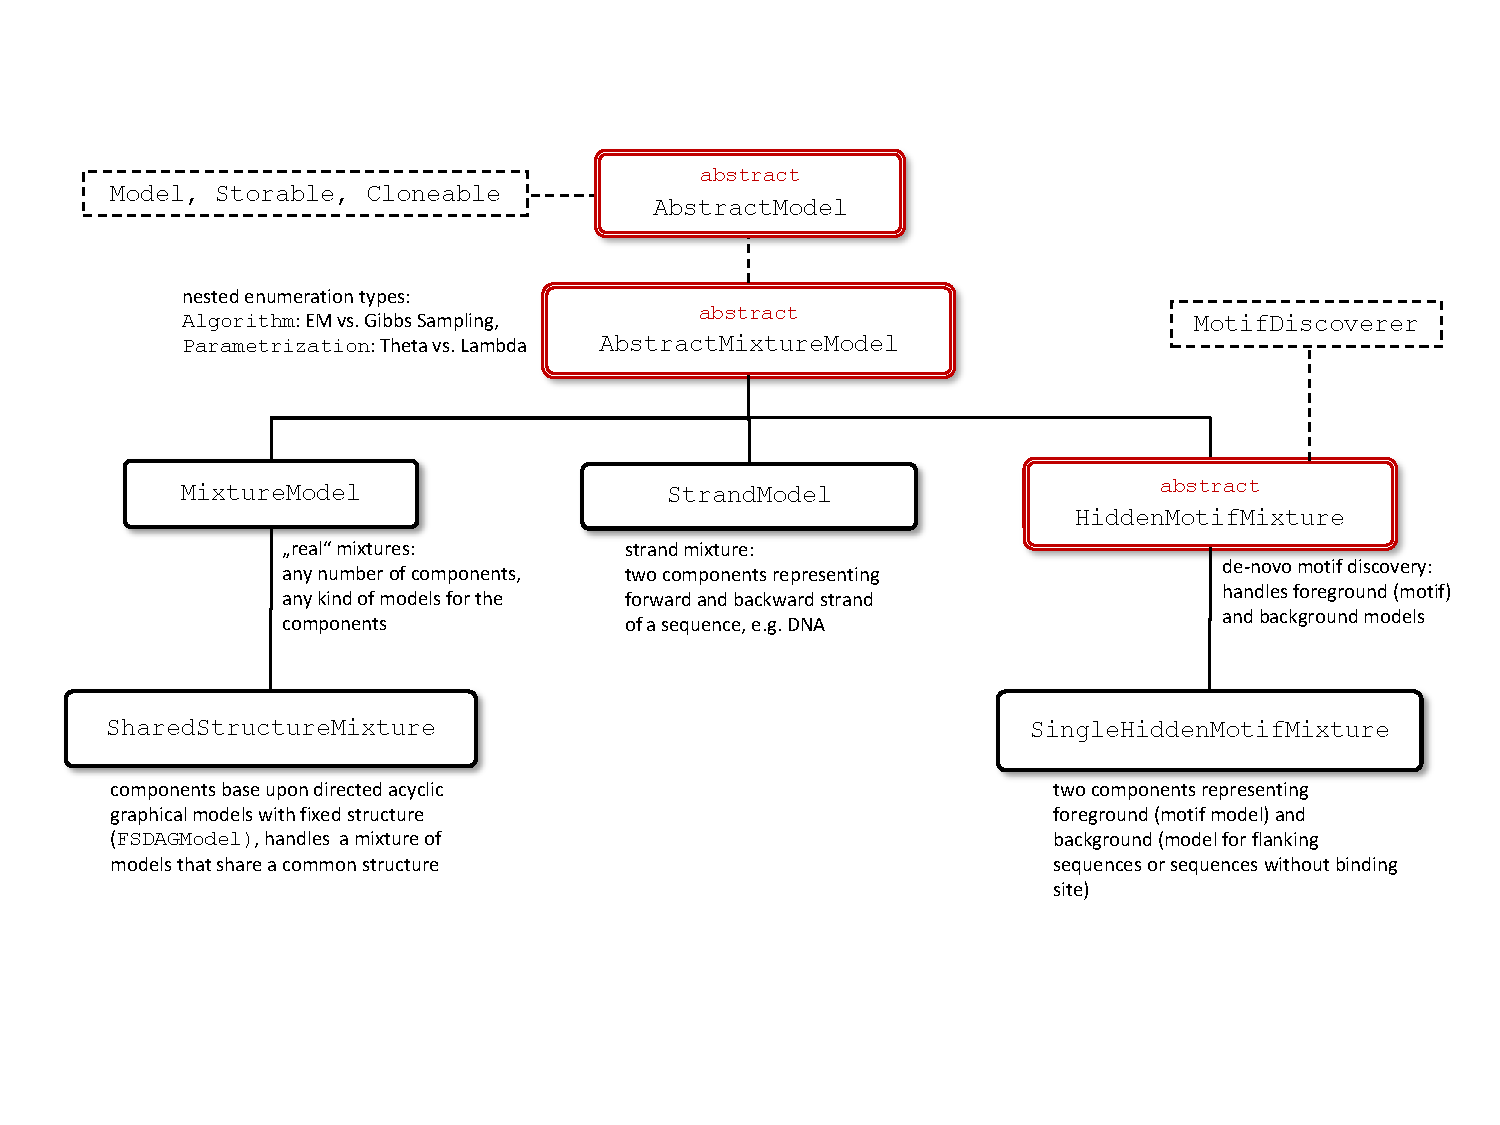
\includegraphics[width=\textwidth]{structure}
\caption{The class hierarchy of mixture model implementations in \jstacs.}\label{fig:class-hierarchy} 
\end{figure}

\section{AbstractMixtureModel}\label{sec:abstractmixture}

The abstract class {\AbstractMixtureModel} is the super class of all mixture models in \jstacs. {\AbstractMixtureModel} extends the
class {\AbstractModel} and is therefore an implementation of {\Storable} and
{\Model}. For this reason, all mixtures can be saved as XML (see \Storable) and hold all features of a probabilistic model, for
instance, it enables the user to train parameters or it can be used in
{\ModelBasedClassifer}.

The parameters of a mixture model are certain probabilities.
As different kinds of parameterization influence the results of
maximum-a-posteriori (MAP) parameter learning, the implementation of
{\AbstractMixtureModel} allows to chose between two parameterizations. This will be explained in detail in the
following section (see section \ref{subsec:params}).

An important point concerning
mixture models is the manner how parameters are trained. In general, training
algorithms for mixture models are iterative algorithms. In {\AbstractMixtureModel}, two iterative algorithms for training of an instance are realized, the EM-algorithm and the sampling of parameters via Gibbs Sampling. More information about that can be found in section \ref{subsec:training}.

\subsection{Parameters}\label{subsec:params}
The parameters of a mixture model consist of the parameters of every
component model and the parameters for the component probabilities.
{\AbstractMixtureModel} and its subclasses are only responsible for the component probabilities whereas the
model parameters are handled by the corresponding component model.

It is important to mention that the estimation of parameter values
with the maximum-a-posteriori (MAP) approach (see also section \ref{subsec:training})
is affected by the chosen parametrization. For this reason,
{\AbstractMixtureModel} allows the user to chose between two kinds
of parametrization. The first parametrization option for the
component probabilities of a mixture model is given by the familiar
$\theta$-parametrization defining $\theta_c := p(c)$ for each component $c$.
The second parametrization is a transformed one which defines $\lambda_c := \log p(c)$ for each component $c$.
When creating a new {\AbstractMixtureModel} the
user can determine in the constructor which parametrization should be used by
specifying the corresponding constant {\href{\APIhome/de/jstacs/models/mixture/AbstractMixtureModel.Parameterization.html#THETA}{THETA}}
or {\href{\APIhome/de/jstacs/models/mixture/AbstractMixtureModel.Parameterization.html#LAMBDA}{LAMBDA}}
defined in the nested enumeration type {\Parametrization}.

\subsection{Training}\label{subsec:training}
The abstract class {\AbstractMixtureModel} provides the possibility
to train the parameters of mixture models by using the EM-algorithm
and Gibbs Sampling. To determine which algorithm should be used the
enumeration type {\Algorithm} nested in this abstract superclass
defines the associated constants
{\href{\APIhome/de/jstacs/models/mixture/AbstractMixtureModel.Algorithm.html#EM}{EM}}
and
{\href{\APIhome/de/jstacs/models/mixture/AbstractMixtureModel.Algorithm.html#GIBBS_SAMPLING}{GIBBS\_SAMPLING}}.
In the same way as the parameterization (see
section \ref{subsec:params}), the training algorithm to
be used has to be specified in the constructor.

The training of the parameters of a mixture model uses the following steps.
First, the sequence component weights for each sequence are computed by the corresponding
mixture model and second, new parameter values are
determined using these weights. The parameters of the component probabilities
are determined by the mixture model, whereas the parameters for each component
are determined by the component model using the train-method.

The algorithms
available for training are iterative algorithms which require the initialization of the parameter values, i.e. the component weights\footnote{It is also possible to hold the component probabilities fixed by specifying certain weights in the constructor. If this is the case, the component probabilities are not considered during the parameter training.}.

Depending on the particular training algorithm there are different ways to
initialize the parameters. For training, using the EM-algorithm, the
component weights are initialized by random values drawn from a
Dirichlet distribution generated by
{\href{\APIhome/de/jstacs/utils/random/DirichletMRG.html}{DirichletMRG}}.
In case of using Gibbs Sampling, the initialization is done by
randomly assigning the weight 1 to exactly one component and 0 to
the rest. This is done by the random generator
{\href{\APIhome/de/jstacs/utils/random/SoftOneOfN.html}{SoftOneOfN}}.

When using the EM-algorithm, it is possible
to decide whether to maximize the Likelihood (ML) or the Posterior
(MAP). The user can switch between these two maximization approaches
by specifying the values in the array for the hyperparameters of the
prior distribution of the component weights in the constructor and by specifying the hyperparameters of the component models. If all hyperparameters are zero likelihood will be maximized, if all hyperparameters are positive the obtained parameters values result from maximization the a-posteriori distribution.
 
In the case of using Gibbs Sampling the component models of the mixture have to implement the interface
{\GibbsSamplingComponent}. Currently, there is a directed acyclic graphical
model with fixed structure implemented that can be used for Gibbs Sampling,
namely the
{\href{\APIhome/de/jstacs/models/mixture/gibbssampling/FSDAGModelForGibbsSampling.html}{FSDAGModelForGibbsSampling}}. 
For the Gibbs Sampling algorithm, it is possible to determine a test of the length of the burn-in phase. The abstract superclass
{\BurnInTest} and its abstract derivation {\AbstractBurnInTest}
define the necessary features and methods for such a test. The
{\href{\APIhome/de/jstacs/models/mixture/gibbssampling/VarianceRatioBurnInTest.html}{VarianceRatioBurnInTest}}
is implemented so far. It calculates the number of initial iterations of a
multi-chain Gibbs Sampling (number of chains > 2) by comparing the variances between the different chains with the variances within the
chains. This test returns the same length of the burn-in phase for all sampled chains.

Using Gibbs Sampling, the sampled parameters are stored in temporary files on the disk, which will be removed by the garbage collector if it is called explicitly at the end of the main method.

\section{Existing Implementations}\label{sec:implementation}
The abstract classes
{\AbstractMixtureModel} and {\HiddenMotifMixture} are implemented for the use of
mixture models whereas the latter is directly derived from {\AbstractMixtureModel} and forms the main class for
all purposes of motif discovery.

Concrete derivations of the superclasses mentioned above are {\MixtureModel} and {\SharedStructureMixture} for ``real'' mixtures, i.e., the mixing of any number of any statistical models, {\StrandModel} for sequences that can be located on
different strands as for instance transcription factor binding sites which can be located on both strands of a double-stranded DNA sequence, and {\SingleHiddenMotifMixture} for detection of a single motif in a sequence.

All these classes will be described more detailed in the following subsections. The class hierarchy which shows the
relations between the different classes is illustrated in Figure \ref{fig:class-hierarchy}.

\subsection{Real mixtures}
``Real'' mixtures of {\Model}s, i.e., mixtures of any number of
any kind of statistical models, are implemented in the class {\MixtureModel}
which directly extends the abstract superclass {\AbstractMixtureModel}. It provides the possibility to mix any
number of any implementation of the interface {\Model}.

The subclass {\SharedStructureMixture} handles a mixture of models with
the same structure that is learned via EM. The mixture components
base upon directed acyclic graphical models with fixed structure
({\FSDAGModel}). Currently, the parameter training is limited to the
EM-algorithm caused by the problem of sampling the graph structure.

\subsection{Strand mixture}
Strand mixture models are for handling sequences that can be located on the
forward or the reverse complementary strand. For this purpose the concrete class
{\StrandModel} is implemented as a direct subclass of
{\AbstractMixtureModel}. Sequences used in the {\StrandModel} have
to be reverse complementable.\footnote{This is ensured by using an
{\href{\APIhome/de/jstacs/data/AlphabetContainer.html}{AlphabetContainer}} with one
{\href{\APIhome/de/jstacs/data/alphabets/ComplementableDiscreteAlphabet.html}{ComplementableDiscreteAlphabet}s}
that is able to compute the reverse complement of a sequence.} For this reason
it is recommended to use this model for DNA sequences but it is not restricted to it. The {\StrandModel} is comprised of exactly two components representing the forward and the reverse complementary strand, respectively.
These components are modeled with the same statistical {\Model}, so
the user has to specify in the constructor only one {\Model} that is
used for both components. The {\StrandModel} is often used for de-novo motif
discovery which is described in the next subsection.

\subsection{De-novo motif discovery}
The abstract class {\HiddenMotifMixture} and its subclass
{\SingleHiddenMotifMixture} are implementations for generative de-novo motif
discovery in sequences.

The main class for de-novo discovering of motifs is {\HiddenMotifMixture}. It is directly derived from the abstract
superclass {\AbstractMixtureModel} and implements the interface
{\MotifDiscoverer}.

{\SingleHiddenMotifMixture}s comprise of two components which
represents the {\Model} for the motif and the {\Model} for the sequence
background, respectively. This mixture model handles sequences
containing exactly one binding site and sequences containing no
binding site. By fixing the component probabilities in the
constructor the user is enabled to train the model either
``\textbf{o}ne \textbf{o}ccurrence \textbf{p}er \textbf{s}equence''
(=OOPS) or ``\textbf{z}ero \textbf{o}r
\textbf{o}ne \textbf{o}ccurrence \textbf{p}er \textbf{s}equence'' (=ZOOPS).
\end{document}
